\documentclass[12pt,a4paper]{report}
\usepackage{amsmath}
\usepackage{amsfonts}
\usepackage{amssymb}
\usepackage{graphicx}
\usepackage{multicol}
\usepackage[utf8]{inputenc}
\usepackage{array}
\usepackage{lipsum}
\graphicspath{{images/}}
\usepackage{parskip}
\usepackage{indentfirst}
\usepackage{courier}
\usepackage{titlesec}
\usepackage{wrapfig}
\usepackage{caption}
\usepackage[left=1.5in, right=1in, top = 1in, bottom = 1in]{geometry}
\usepackage{float}
\usepackage[ruled]{algorithm}
\usepackage{algpseudocode}
\usepackage{graphicx}
\usepackage{url}
\usepackage{rotating}

\geometry{headheight = 12pt}
\parindent 15pt
\parskip 2ex

\usepackage{listings}
\usepackage{color}
\definecolor{lightgray}{rgb}{.9,.9,.9}
\definecolor{darkgray}{rgb}{.4,.4,.4}
\definecolor{purple}{rgb}{0.65, 0.12, 0.82}

\lstdefinelanguage{JavaScript}{
	keywords={typeof, new, true, false, catch, function, return, null, catch, switch, var, if, in, while, do, else, case, break},
	keywordstyle=\color{blue}\bfseries,
	ndkeywords={class, export, boolean, throw, implements, import, this},
	ndkeywordstyle=\color{darkgray}\bfseries,
	identifierstyle=\color{black},
	sensitive=false,
	comment=[l]{//},
	morecomment=[s]{/*}{*/},
	commentstyle=\color{purple}\ttfamily,
	stringstyle=\color{red}\ttfamily,
	morestring=[b]',
	morestring=[b]"
}

\lstset{
	language=JavaScript,
	backgroundcolor=\color{lightgray},
	extendedchars=true,
	basicstyle=\footnotesize\ttfamily,
	showstringspaces=false,
	showspaces=false,
	numbers=left,
	numberstyle=\footnotesize,
	numbersep=9pt,
	tabsize=2,
	breaklines=true,
	showtabs=false,
	captionpos=b
}

\usepackage{filecontents}

\begin{filecontents}{\jobname.bib}
	@ARTICLE{Dudarev1998,
		author = {Dudarev, S. L. and Botton, G. A. and Savrasov, S. Y. and Humphreys,
			C. J. and Sutton, A. P.},
		title = {Electron-energy-loss spectra and the structural stability of nickel
			oxide: An LSDA+U study},
		journal = {Phys. Rev. B},
		year = {1998},
		volume = {57},
		pages = {1505--1509},
		month = {Jan},
		doi = {10.1103/PhysRevB.57.1505},
		number = {3},
		publisher = {American Physical Society},
		url = {http://link.aps.org/doi/10.1103/PhysRevB.57.1505}
	}
	@ARTICLE{Dudarev1997,
		author = {Dudarev, S. L. and Botton, G. A. and Savrasov, S. Y. and Humphreys,
			C. J. and Sutton, A. P.},
		title = {Electron-energy-loss spectra and the structural stability of nickel
			oxide: An LSDA+U study},
		journal = {Phys. Rev. B},
		year = {1998},
		volume = {57},
		pages = {1505--1509},
		month = {Jan},
		doi = {10.1103/PhysRevB.57.1505},
		number = {3},
		publisher = {American Physical Society},
		url = {http://link.aps.org/doi/10.1103/PhysRevB.57.1505}
	}
\end{filecontents}

\algblockdefx[ClassBlock]{Class}{EndClass} [1]{\textbf{class} #1} [0]{}
\algtext*{EndClass}

\newcommand{\WRP}{\par\qquad\(\hookrightarrow\)\enspace}

\renewcommand{\listfigurename}{Figures}
\renewcommand{\listtablename}{Tables}

\titleformat{\chapter}[display]   
{\normalfont\huge\bfseries}{\chaptertitlename\ \thechapter}{20pt}{\Huge}   
\titlespacing*{\chapter}{0pt}{-50pt}{20pt}

\author{Group 42 \\ -------------------- \\Jacob Spigle, Zachary Painter, David Akridge, Hunter Figueroa}
\title{Critical Encounters}

\begin{document}
	
	\newpage
	\section{Hunter Figueroa}
	\begin{wrapfigure}{l}{0\textwidth}
		
\includegraphics[scale=0.05]{Hunter_Figueroa}
	\end{wrapfigure}
	I have been playing tabletop role-playing games for over 6 years now. They served as a creative outlet where I could experiment with new creative ideas. I prefer acting as a DM, I’ve only played a single session as a player, I loved the idea of being all powerful creator of a world that I could share with my friends. The tabletop community, namely the Dungeon \& Dragons community is like no other that I have seen before. It is composed of highly talented, highly cooperative  and interactive people who do their very best to better and expand the role playing community. For close to two years now I have put a considerable about of my free time into constructing a digital service to help this same cause. So when I heard Jacob pitch this idea, I knew it was the one for me. We’ve got something really special here, and with the team that we have I feel we can create something game changing.
	
	\chapter*{User Interface}
	\stepcounter{chapter}
	\addcontentsline{toc}{chapter}{User Interface}
	\section{Overall Design and Navigation Bar}
	\begin{figure}[H]
		\centering
		\centerline{
\includegraphics[scale=.30]{navbar}}
		\caption{NavBar}
		\label{fig: NavBar}
	\end{figure}
	\section{Registration Page}
	\begin{figure}[H]
		\centering
		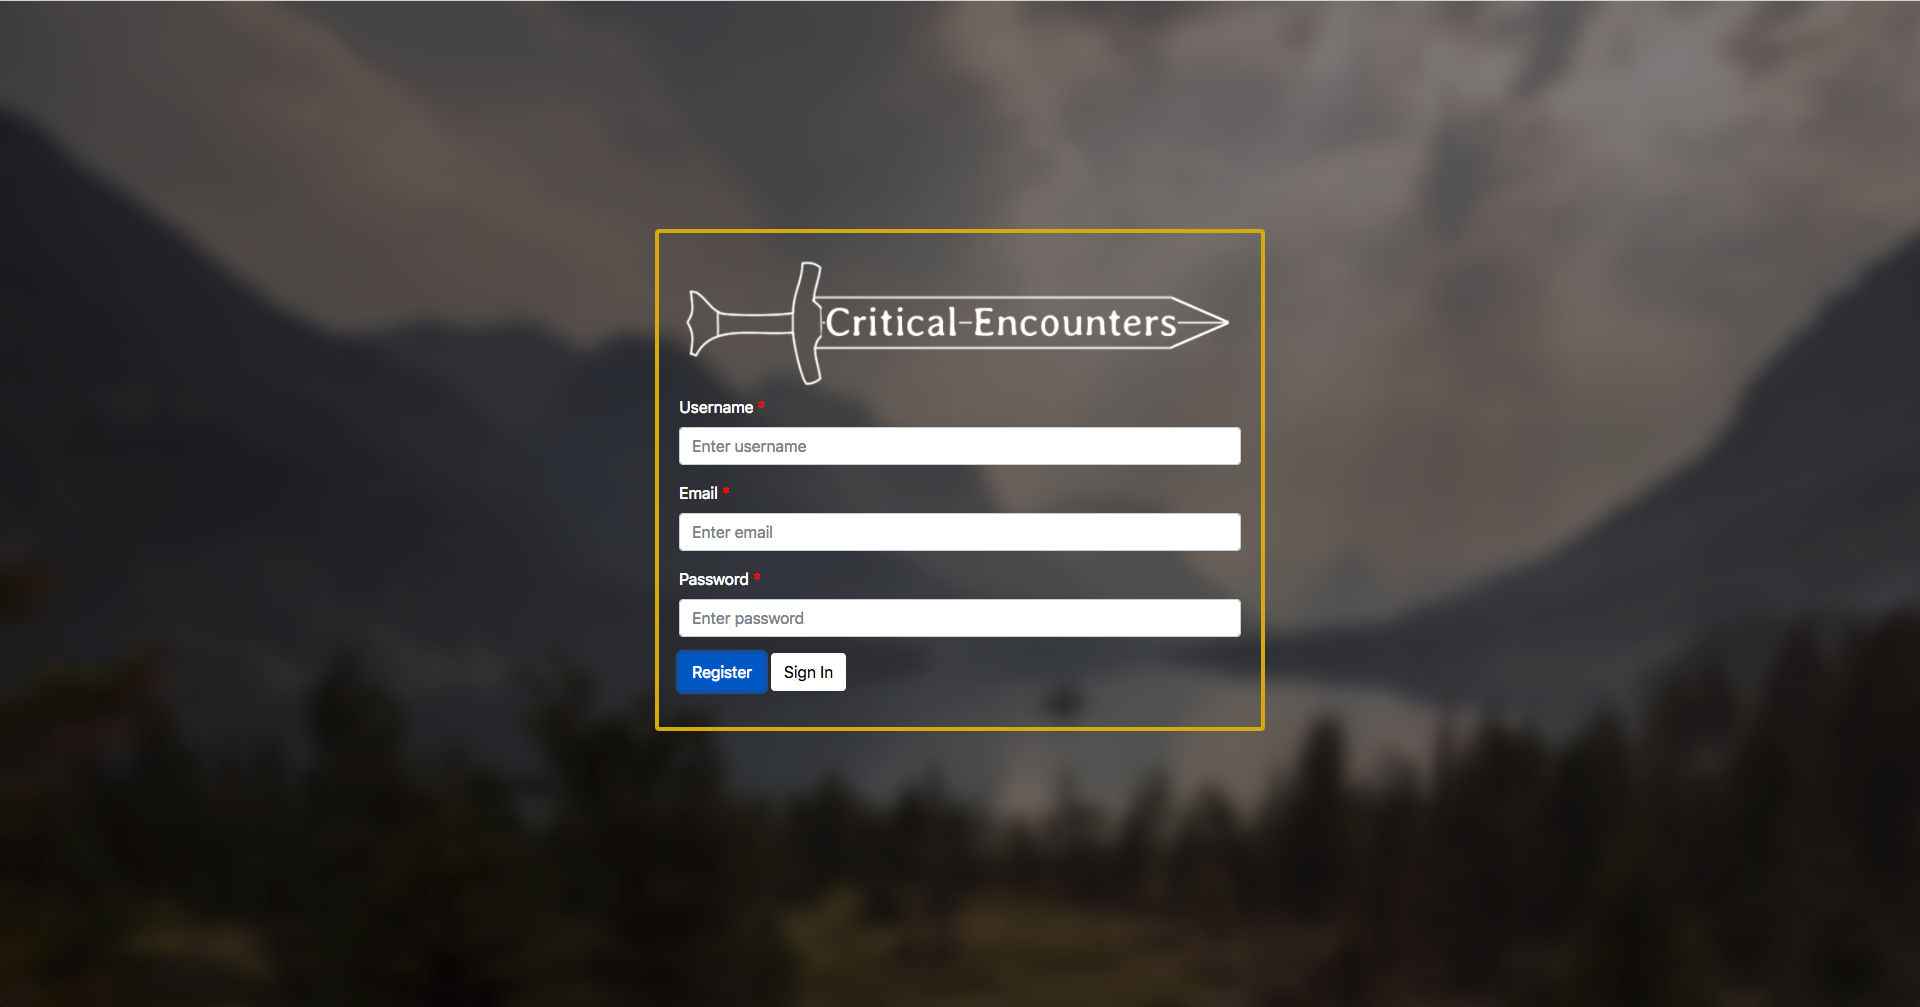
\includegraphics[scale=.20]{register}
		\caption{Registration Page}
		\label{fig: Registration Page}
	\end{figure}
	\section{Login Page}
	\begin{figure}[H]
		\centering
		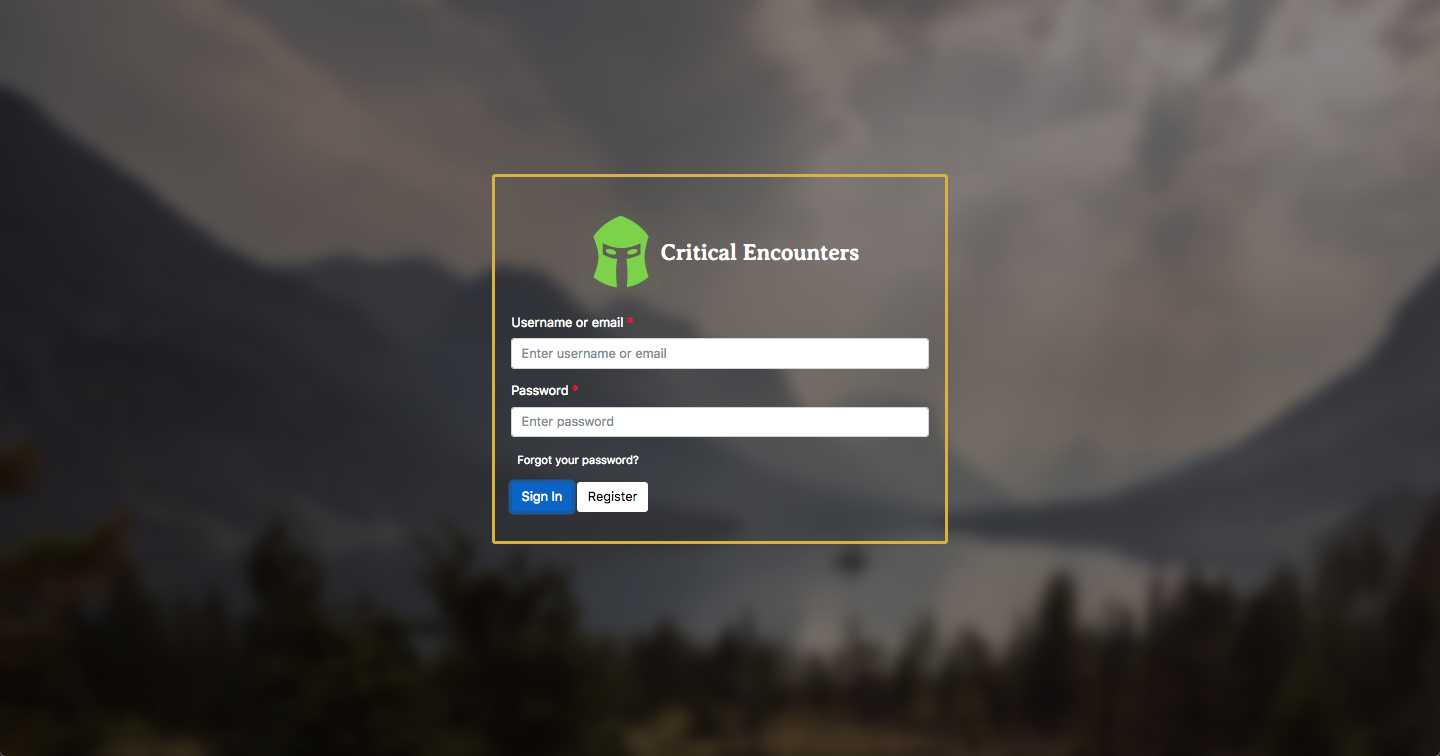
\includegraphics[scale=.20]{login}
		\caption{Login Page}
		\label{fig: Login Page}
	\end{figure}
	\section{Dashboard}
	\begin{figure}[H]
		\centering
		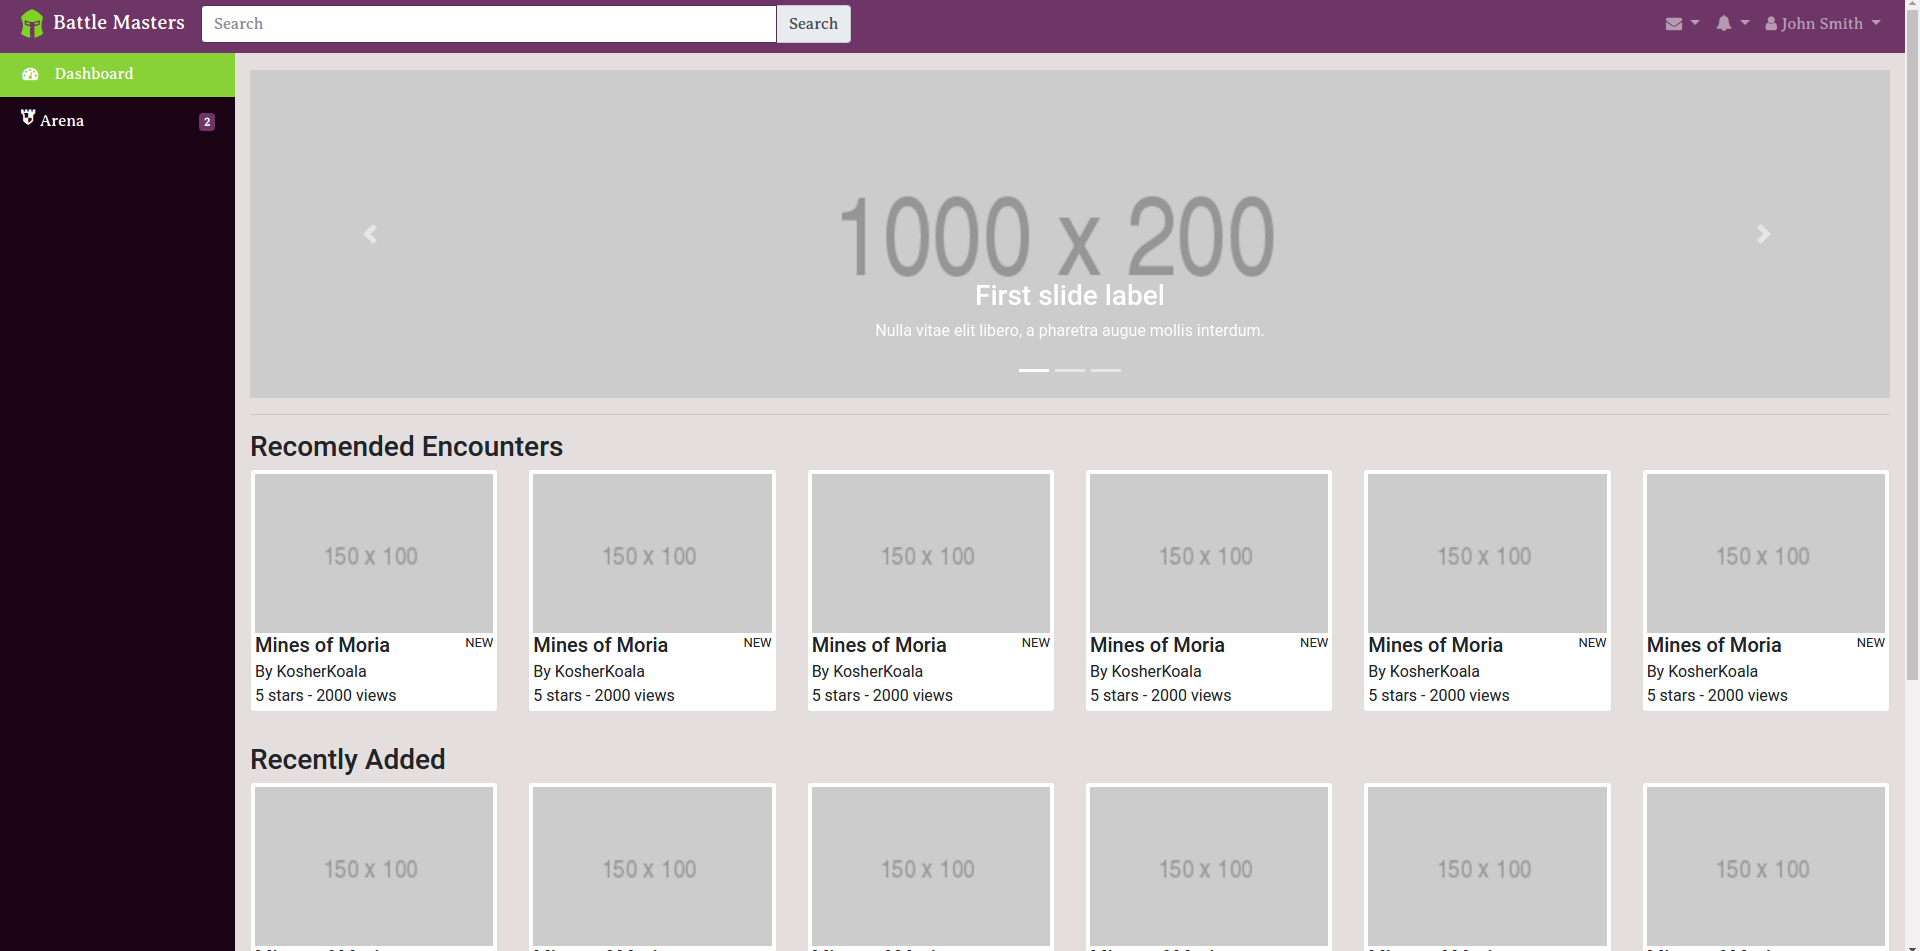
\includegraphics[scale=.20]{home}
		\caption{Dashboard}
		\label{fig: Dashboard}
	\end{figure}
	\section{Encounter Browser}
	\begin{figure}[H]
		\centering
		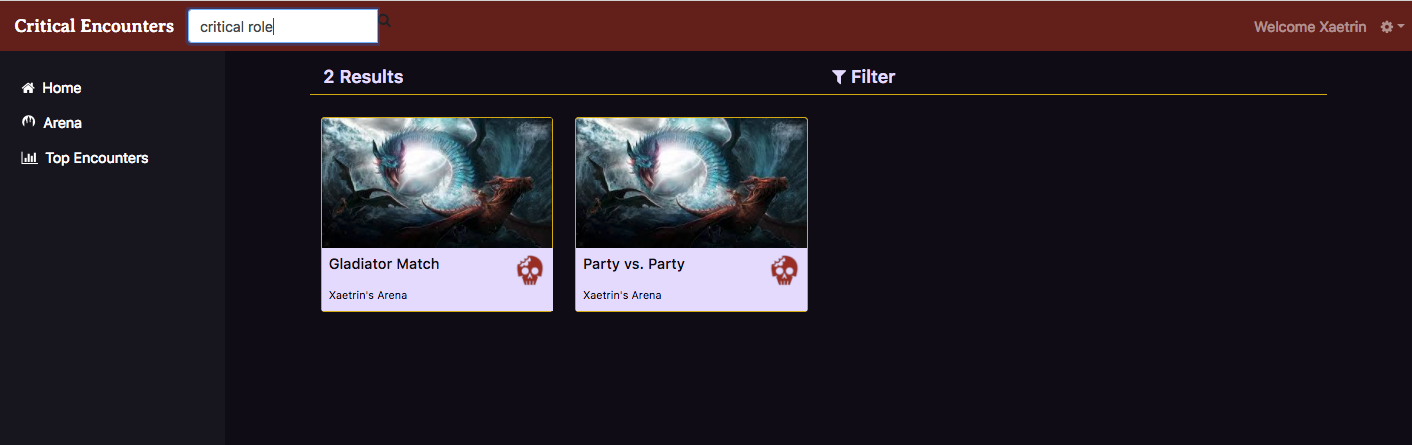
\includegraphics[scale=.19]{search}
		\caption{Encounter Browser}
		\label{fig: Encounter Browser}
	\end{figure}
	\section{Arena}
	\begin{figure}[H]
		\centering
		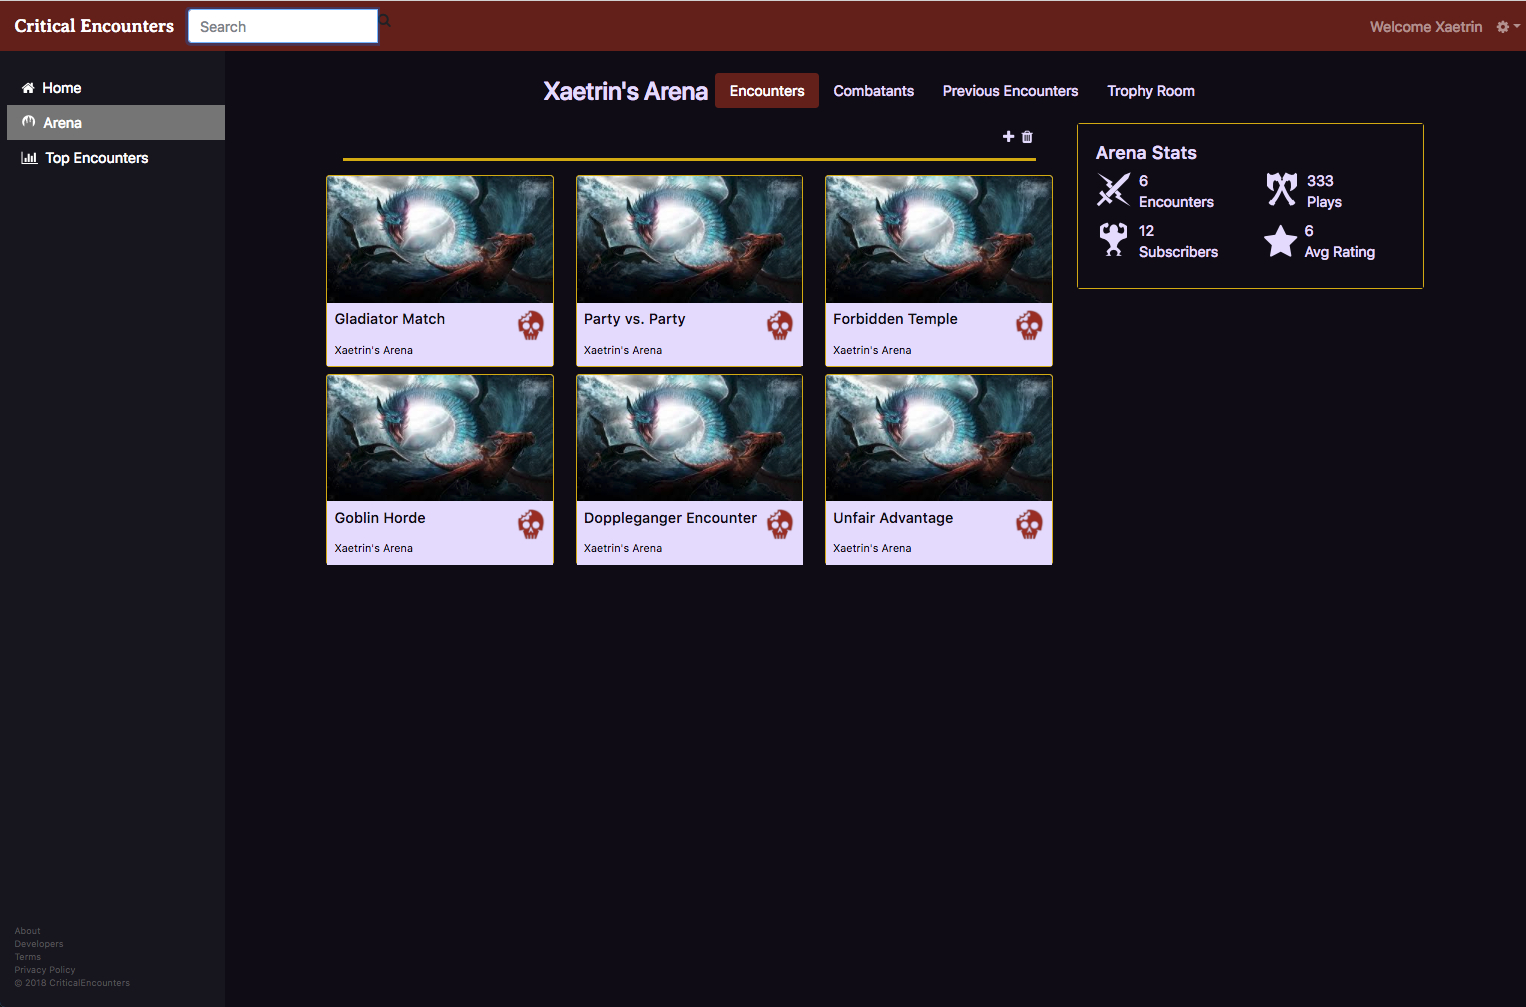
\includegraphics[scale=.20]{arena}
		\caption{Arena}
		\label{fig: Arena}
	\end{figure}
	\section{Encounter Page}
	\begin{figure}[H]
		\centering
		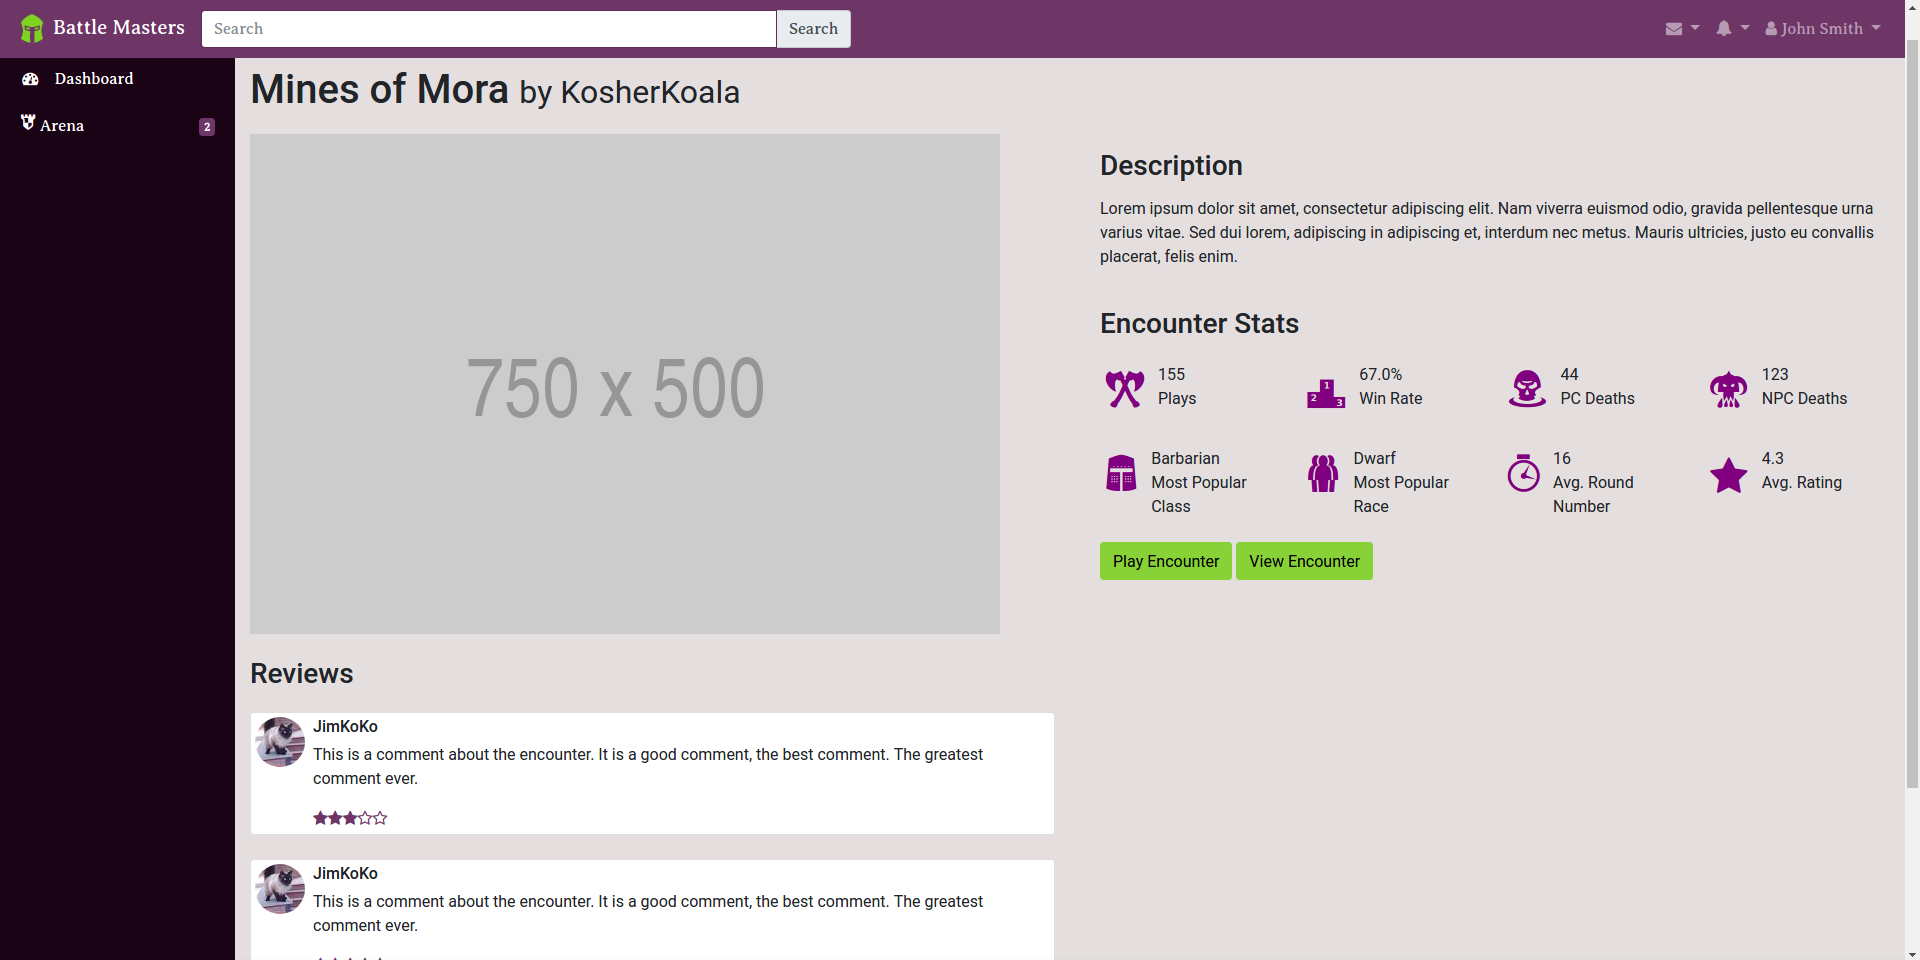
\includegraphics[scale=.20]{encounter}
		\caption{Encounter Page}
		\label{fig: Encounter Page}
	\end{figure}
	
	\newpage
	\section{Battlefield}
	The Battlefield is arguably the most important and most challenging frontend development we must complete. The Battlefield is where users will create, edit, and play their encounters. Because of its importance we have put a lot of thought into the requirements, design, and implementation plans. Both the frontend and backend are working closely on this component because the battlefield is the stage that our AI will be able to show its capabilities.
	\begin{figure}[H]
		\centering
		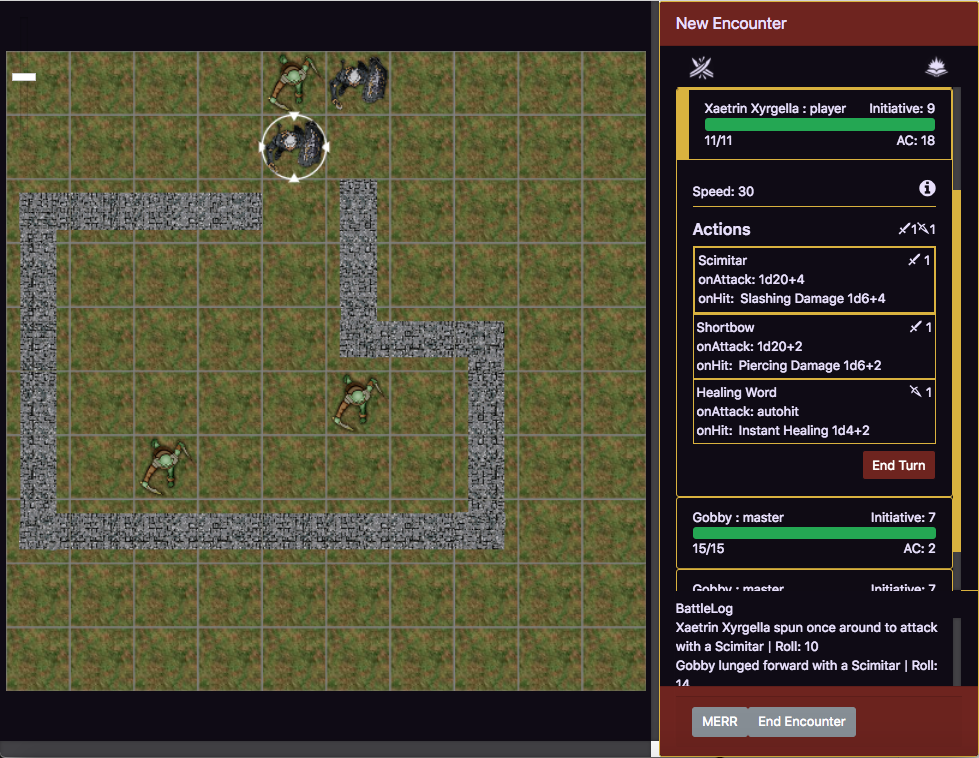
\includegraphics[scale=.5]{encountercreator}
		\caption{Battlefield Prototype}
		\label{fig: Battlefield Prototype}
	\end{figure}
	Above is a early prototype of our Battlefield. It contains three separate components: the main battle board, the sidebar, and the combat log. 
	\subsection {The Battle Board }
	The Battle Board is where all the environment, obstacles, and combatants are rendered. The board is a 2d top down arena, inspired by popular strategy games such as Civilization. The board is composed of checkerboard likes faces Each of which represent 5 feet of space in the game world. Obstacles and combatants will be rendered inside of these spaces. Obstacles and combatants can be hovered over and selected as well as click and drag into other spaces within the combatants movement range. If one of the combatants or obstacles are clicked their details and descriptions will appear in the sidebar. 
	\begin{figure}[H]
		\centering
		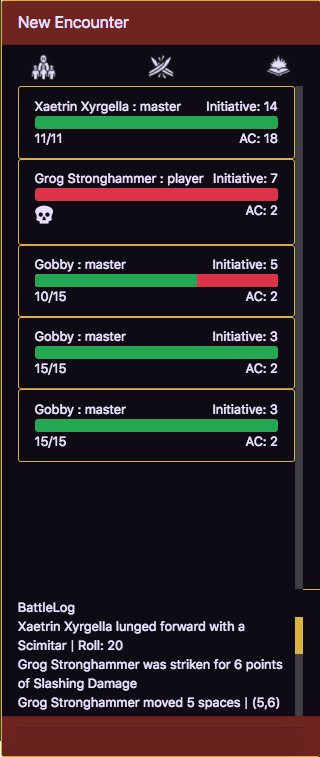
\includegraphics[scale=.5]{encountercreatorsidebar}
		\caption{Battlefield Prototype Sidebar}
		\label{fig: Battlefield Prototype Sidebar}
	\end{figure}
	\subsection {The Sidebar }
	In the sidebar the user can view a combated or obstacles description and statistics. If the user selected a combatant the user will also be able to browse the combatants actions and on the combatants turned use those actions in combat. The sidebar is also where the user will control his combatant honest turn in combat whether it involves rolling initiative, performing actions, adjusting equipment and stats, or ending the turn itself. The sidebar will also be used in the creation mode of the battlefield. In the sidebar the user will be able to search, select, in drag combatants and obstacles onto the battlefield. They can also view and edit any of the stats using a form contained in the sidebar. The sidebar will also be where the user can make adjustments to combatant AI whether it's setting its aggressiveness level or selecting one of our built in my presets. In other words the sidebar is where the user will manage all the details of the encounter in both creation and playing modes. 
	\subsection {The Battlelog }
	The Battlelog below is where all of the messages attached to combat an encounter actions will be displayed. They will supply the user with an up-to-date text rendition of the encounter. It will include messages like, "The Goblin struck the cleric with a sword dealing 5 points of slashing damage", "The wizard casted Firebolt at the ogre but it missed", and "The Rogue hides behind the barrel the dragon does not seem to notice him". Early on in the Battlelog implementation we plan for very simple straightforward statistical messages that will aid us during testing and AI development. However we are planning to expand this feature to aid in role-play. We feel that having more colorful destruction of the actions occurring in the encounter. Will add another layer of fun for the user. 
	\subsection {States and Controllers }
	The same battle components will be used for both creation of the encounters and playing of the encounters. The controller will either hide or allow the user to view certain tools depending on what state the user has entered the battlefield in. For example if the user was in creation mode, they would also have access to our database of built-in combatants and obstacles said they will be able to add to their encounter. 
	\subsection {Future Implementation/Design Plans }
	Stated earlier this is a early prototype created in Angular 4 using Bootstrap for the UI. We plan on porting the system over to React and using fabricjs and HTML5 canvas to construct the Battle Board. This will give us a lot more freedom with red during the environment including varied combating in obstacle sizes and easier drag-and-drop capabilities. We also plan for the battlefield to take out the entirety of the players Street. The sidebar and the Battlelog themselves will be toggleable by clickable buttons on the sides and bottom of the screen. The battlefield will exist on its own component separate from the rest of the site so the overlaying UI such as the header and sidebar of the main site will not interfere with the battlefield experience.
	\newpage
	\section{Color Scheme}
	\begin{figure}[H]
		\centering
		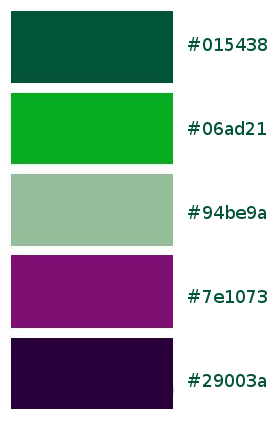
\includegraphics[scale=.5]{colors}
		\caption{Color Scheme}
		\label{fig: Color Scheme}
	\end{figure}
	When choosing a color palette to build our website, we looked around at other websites that focused on role-playing game topics and at gaming sites as well. The majority of these sites opt for a black and red or some combination black and X style when creating their look and feel. With Critical Encounters we wanted to break a little bit out of the norm and use colors that really pop out at the user, really make an impression on them, and set ourselves a bit apart from the other cites that they have been to.

	\newpage
	\subsection {Logo}
	\begin{figure}[H]
		\centering
		
\includegraphics[scale=.5]{logo-large}
		\caption{Critical Encounters' Logo}
		\label{fig: Critical Encounters' Logo}
	\end{figure}
	We wanted the logo design to accompany the overall UI design choices of the website with a more simplistic approach, while also representing the RPG aspect of Critical Encounters. We decided on a helmet because it gave a little more of a human feel, we thought swords or other weapons would be too inanimate and maybe even a bit cliché. Because of the light green color, and the contrast of our darker purple color choice with the navigation bar, this logo will "pop" on all of the views on the website(Figure \ref{fig: Critical Encoutners' Logo with Background}). The logo can also be easily scaled to fit most container sizes, which fits in to our application's versatility between desktop and mobile browsers.


	
	\newpage
	\chapter*{Application Design}
	\stepcounter{chapter}
	\addcontentsline{toc}{chapter}{Application Design}
	\section {High Level Design}
	\begin{figure}[H]
		\centering
		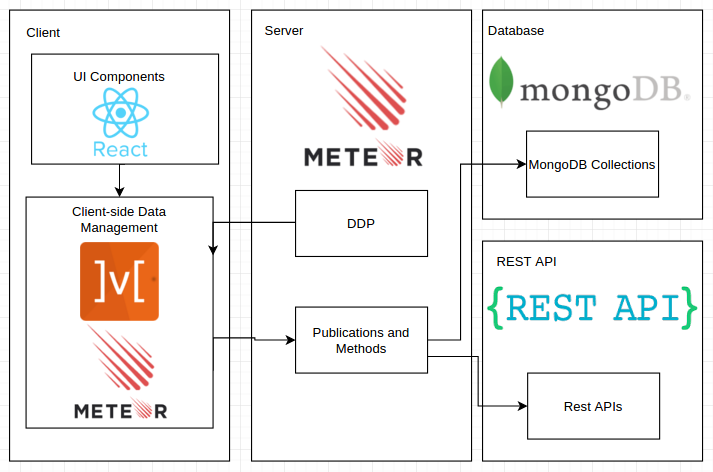
\includegraphics[scale=.5]{designsd.png}
		\caption{High Level Design Diagram}
		\label{fig: High Level Design}
	\end{figure}
	
	\paragraph{}We will be implementing a Client-Server Design structure that is commonly used with web apps such as Critical Encounters. There are three areas of production in this high-level design: Server, Database/Rest API and Client-Side. The UI components will be developed in REACT and will control the the MVC system. Data management on the client-side will be managed by MobX and Meteor, the latter of which will server as the point of contact with the server-side of the app. The server will also be developed in Meteor, and will be responsible for contacting the database, developed in MongoDB and performing REST API commands when necessary. \par
	The relationship between client and server will be a sudo model-view-controller architecture. Where REACT will act as the as application's view and Meteor/MobX will act as both the controller and the model. Meteor with MobX will automatically manage the data flow, client state, and client rendering.
	
	\section {Design Patterns}
	
	\begin{figure}[H]
		\centering
		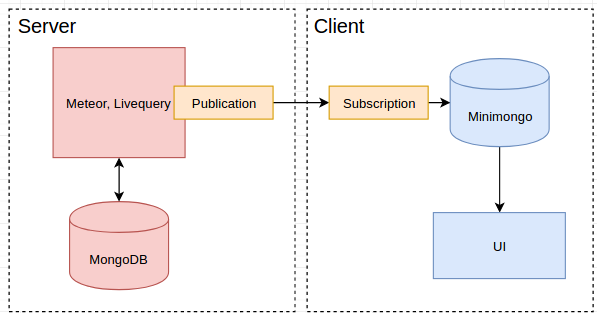
\includegraphics[scale=.7]{orm.png}
		\caption{Design Pattern Figure}
		\label{fig: Design Pattern Figure}
	\end{figure}
	
	\paragraph{} Meteor uses implements a ORM/MERN, Object-relational mapping / MongoDB - Express - React, stack design pattern. It focuses on model driven development, in which the models are shared between the server and the client. This is seen most clearly seen in the MiniMongo database cache that is accessible by the font-end front end and can asynchronously update the MongoDb REST API is implemented automatically which translates to automatic database updates.
	
	\newpage
	\section {Server Design}
	\subsection{Meteor}
	\begin{wrapfigure}{l}{0\textwidth}
		
\includegraphics[scale=.2]{meteorJS}
		\caption{Meteor.js}
		\label{fig: Meteor.js}
	\end{wrapfigure}
	Meteor is a full-stack JavaScript platform for developing modern web and mobile applications. Meteor includes a key set of technologies for building connected-client reactive applications, a build tool, and a curated set of packages from the Node.js and general JavaScript community.
	
	
	
	On the client, there is no direct connection to the MongoDB database, and in fact a synchronous API to it is not possible (nor probably what you want). Instead, on the client, a collection is a client side cache of the database. This is achieved thanks to the MiniMongo library—an in-memory, all JS, implementation of the MongoDB API. What this means is that on the client, when you write:
	
	\begin{lstlisting}
	const Users = new Mongo.Collection('users');
	\end{lstlisting}
	
	It creates a new collection in the MongoDB database called 'users' and assigns the collection to the variable Users. Now you can send queries and updates to the database:
	
	\begin{lstlisting}
	// Return an array of useres with name Hunter
	const allUsers = Users.find({ name: 'Hunter' }).fetch();
	
	// Create a new user.
	Messages.insert({ name: 'hunter', email: 'hunter@gmail.com', validated: false });
	
	// Validate user
	Users.update(allUsers[0]._id, { $set: { validated: true } });
	\end{lstlisting}
	
	
	\begin{tabular}{ |p{3cm}||p{3cm}|p{3cm}|p{3cm}|  }
		\hline
		\multicolumn{4}{|c|}{Meteor Database} \\
		\hline
		Country Name     or Area Name& ISO ALPHA 2 Code &ISO ALPHA 3 Code&ISO numeric Code\\
		\hline
		Afghanistan   & AF    &AFG&   004\\
		Aland Islands&   AX  & ALA   &248\\
		Albania &AL & ALB&  008\\
		Algeria    &DZ & DZA&  012\\
		American Samoa&   AS  & ASM&016\\
		Andorra& AD  & AND   &020\\
		Angola& AO  & AGO&024\\
		\hline
	\end{tabular}
	
	\subsection{Server Sequence Diagrams}
	
	\subsubsection {Register SSD}
	\begin{figure}[H]
		\centering
		\centerline{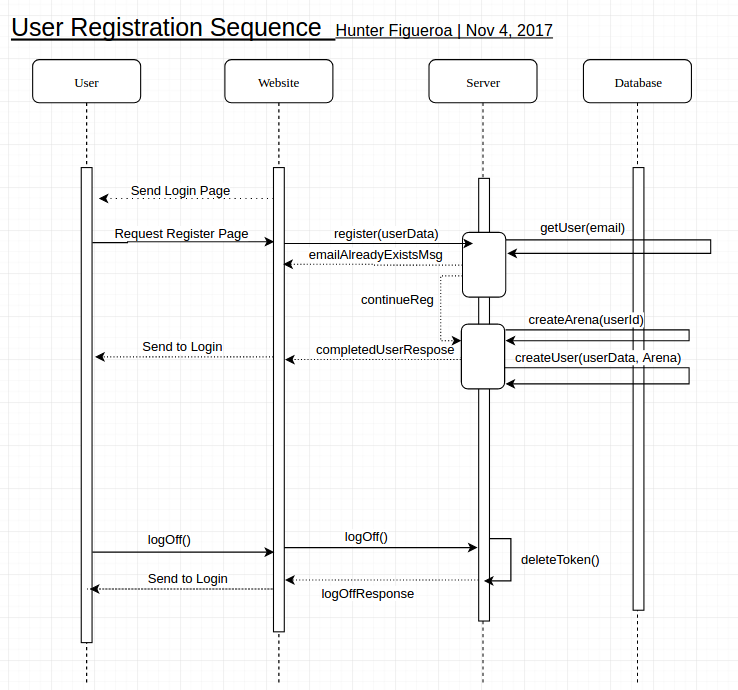
\includegraphics[scale=.7, angle=90]{ssd_register}}
		\caption{User Register SSD}
		\label{fig: User Register SSD }
	\end{figure}
	
	\newpage
	\subsubsection {Encounter Search SSD}
	\begin{figure}[H]
		\centering
		\centerline{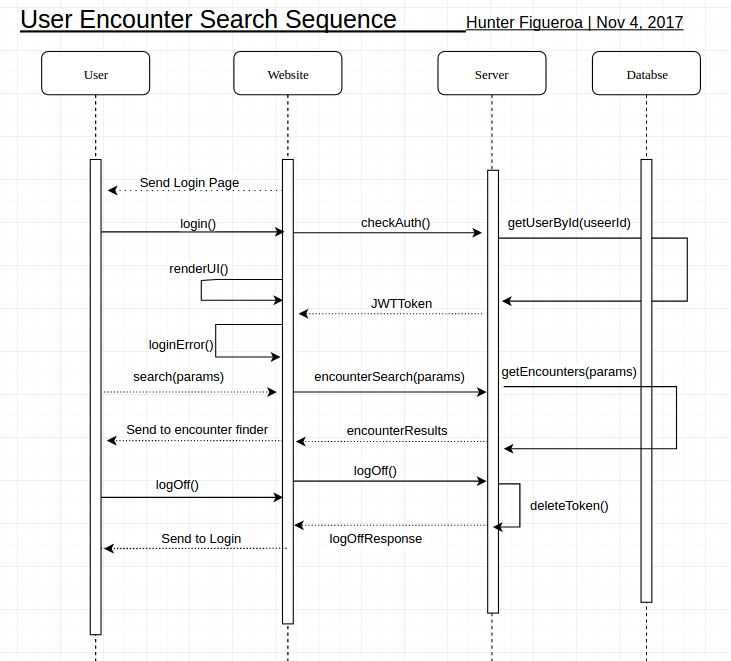
\includegraphics[scale=.7, angle=90]{ssd_encounter_search}}
		\caption{Encounter Search SSD}
		\label{fig: Encounter Search SSD }
	\end{figure}
	
	\newpage
	\subsubsection {Encounter Feed SSD}
	\begin{figure}[H]
		\centering
		\centerline{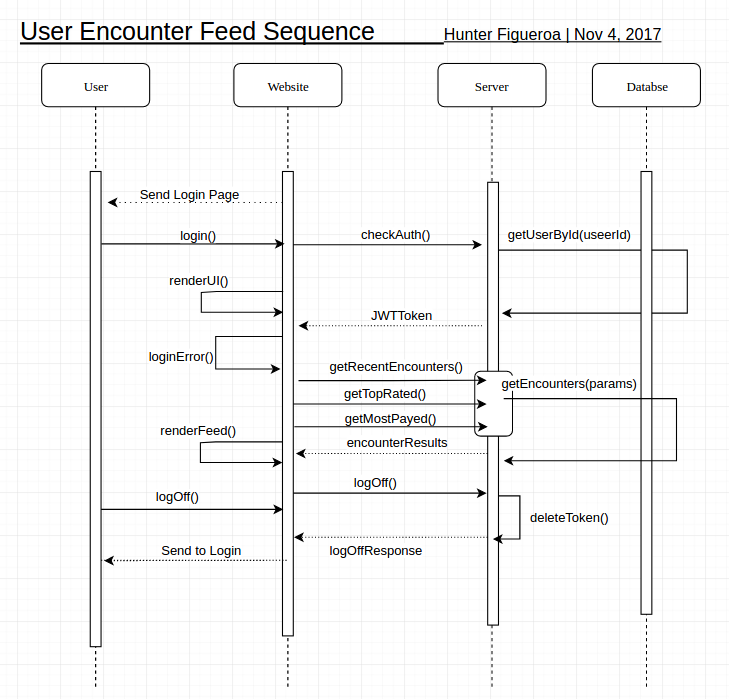
\includegraphics[scale=.7, angle=90]{ssd_encounter_feed}}
		\caption{Encounter Feed SSD}
		\label{fig: Encountner Feed SSD }
	\end{figure}
	
	\newpage
	\subsubsection {Arena Subscription SSD}
	\begin{figure}[H]
		\centering
		\centerline{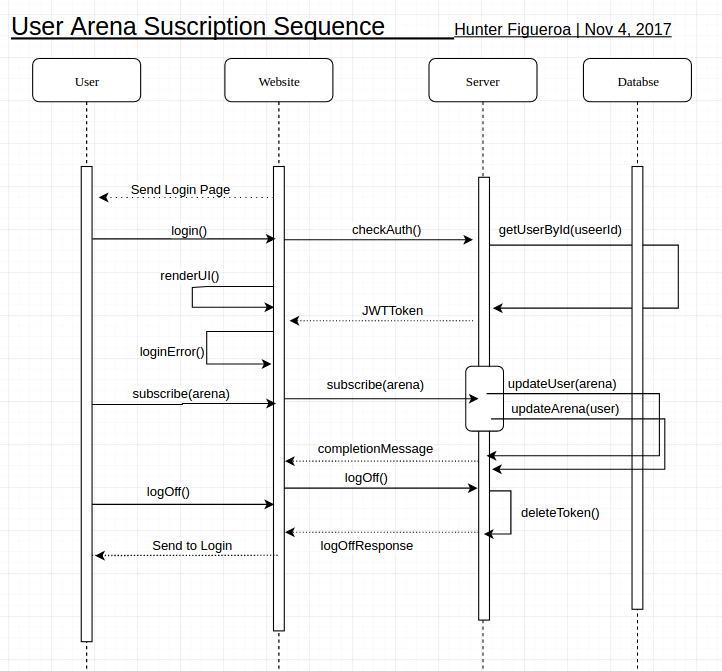
\includegraphics[scale=.7, angle=90]{ssd_subscribe}}
		\caption{Arena Subscription SSD}
		\label{fig: Arena Subscription SSD }
	\end{figure}
	
	\newpage
	\subsection {Encounter Review SSD}
	\begin{figure}[H]
		\centering
		\centerline{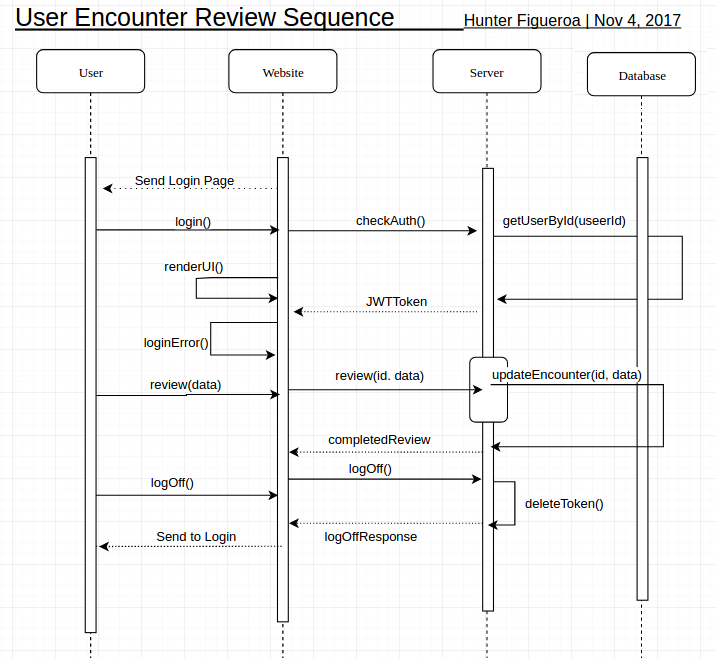
\includegraphics[scale=.7, angle=90]{ssd_review}}
		\caption{Encounter Review SSD}
		\label{fig: Encounter Review SSD }
	\end{figure}
	
	\newpage
	\subsection {Encounter Resources SSD}
	\begin{figure}[H]
		\centering
		\centerline{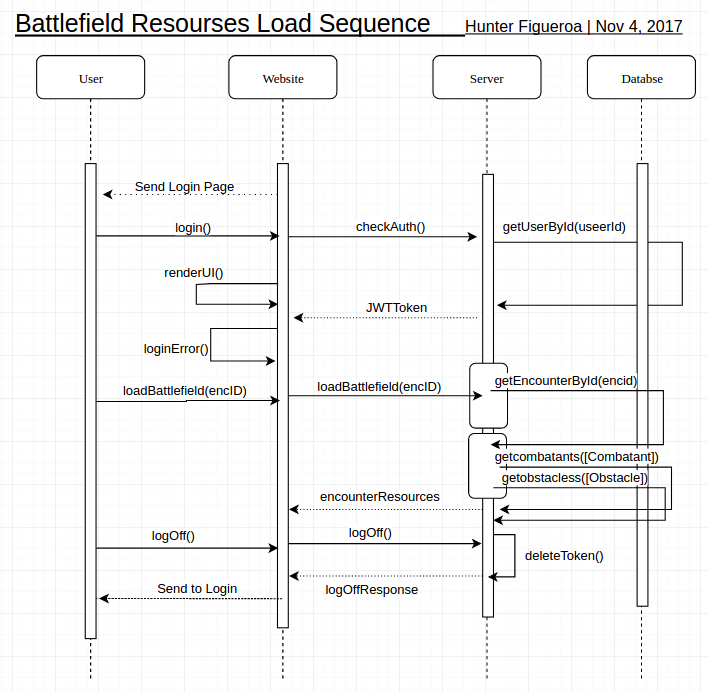
\includegraphics[scale=.7, angle=90]{ssd_resourses}}
		\caption{Encounter Resourses SSD}
		\label{fig: Encounter Resourses SSD }
	\end{figure}
	
	\newpage
	\subsection {Load Arena Page/Data SSD}
	\begin{figure}[H]
		\centering
		\centerline{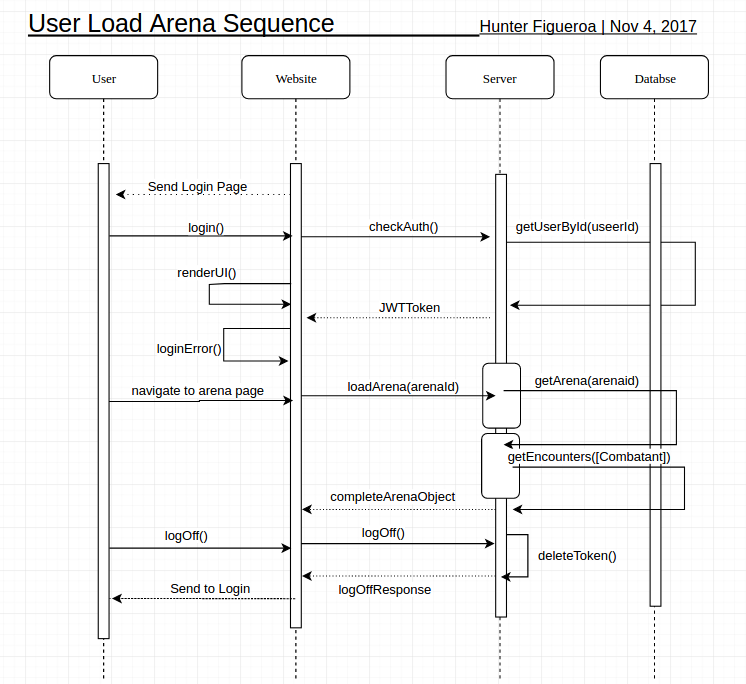
\includegraphics[scale=.7, angle=90]{ssd_arena}}
		\caption{Load Arena Page/Data SSD}
		\label{fig: Load Arena Page/Data SSD }
	\end{figure}
	
	\newpage
	\subsection {Load Encounter Page/Data SSD}
	\begin{figure}[H]
		\centering
		\centerline{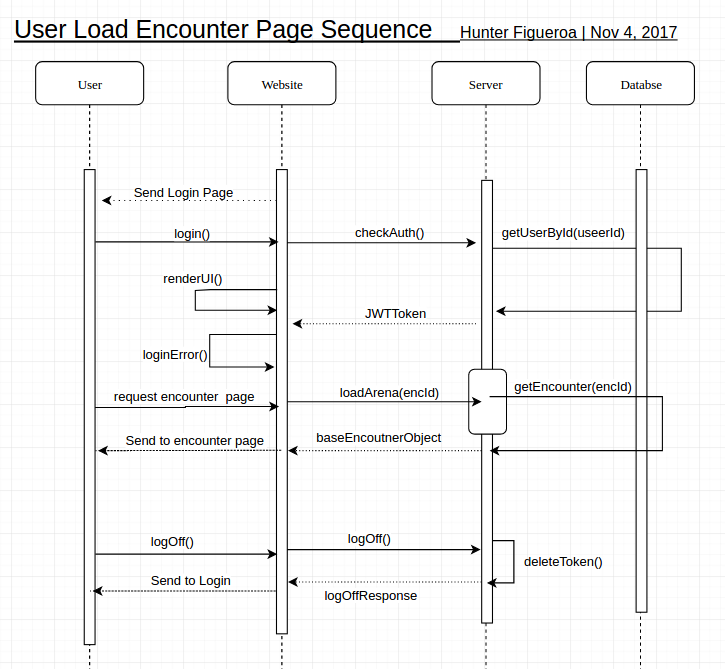
\includegraphics[scale=.7, angle=90]{ssd_encounter_page}}
		\caption{Load Encounter Page/Data SSD}
		\label{fig: Load Encounter Page/Data SSD }
	\end{figure}
	
	\newpage
	\subsection {Create Encounter SSD}
	\begin{figure}[H]
		\centering
		\centerline{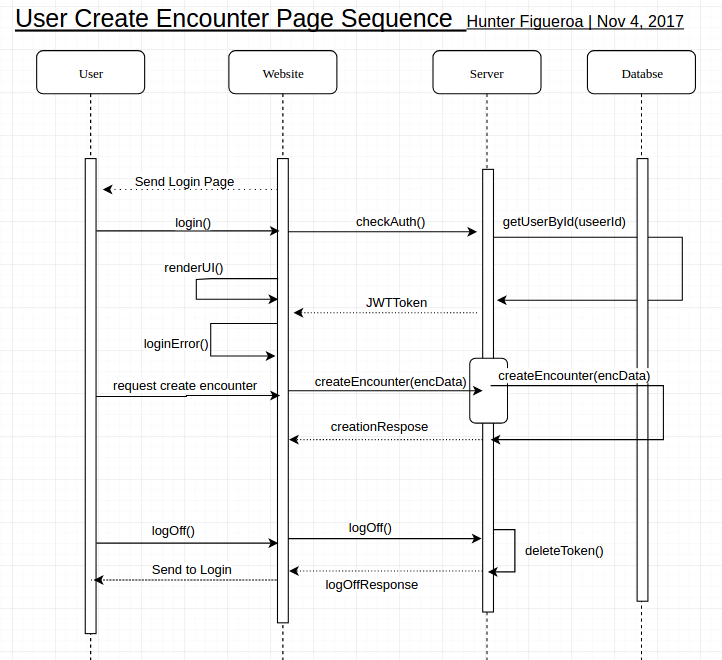
\includegraphics[scale=.7, angle=90]{ssd_create_enc}}
		\caption{Create Encounter SSD}
		\label{fig: Create Encounter SSD }
	\end{figure}
	
	
	\newpage
	\section{Database Design}
	\subsection {Database Diagram}
	\begin{figure}[H]
		\centering
		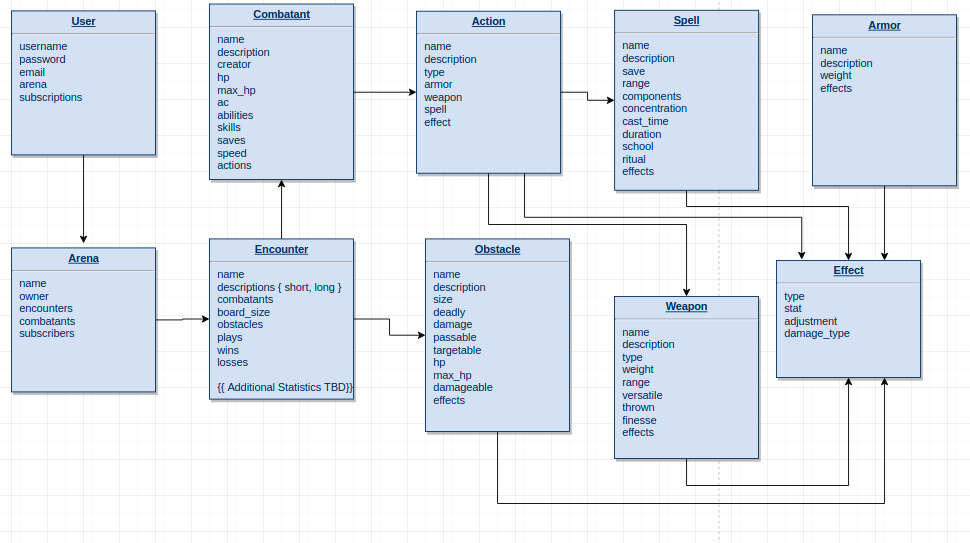
\includegraphics[scale=.4]{database_schema}
		\caption{Databse Schema}
		\label{fig: Databse Schema }
	\end{figure}
	\subsection{Schema}
	Below are schema that will be used to structure the MongoDB collections. The schema themselves will be implemented in Meteor using their MongoDB schema syntax and design. Below is an example of the schema representation of a Critical Encounter user collection:
	
	\begin{lstlisting}
	Users.schema = new SimpleSchema({
	username: {type: String, required: true},
	password: {type: String, required: true},
	arena: {type: String, regEx: SimpleSchema.RegEx.Id},
	subscriptions: [{type: String, regEx: SimpleSchema.RegEx.Id}]
	});
	\end{lstlisting}
	
	The general structure is a field name and a matching feild type (String, Boolean, Object ) with optional requirements or parameters (regEx: SimpleSchema.RegEx.Id).
	
	Note: The { "Collection Name" } notation represents an Object.id that correlates to a MongoDB object of that collection type
	\subsubsection{User Schema}
	\begin{figure}[H]
		\centering
		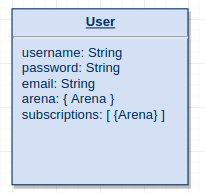
\includegraphics[scale=.75]{schema-user}
		\caption{User Schema}
		\label{fig: User Schema }
	\end{figure}
	
	\paragraph{}This schema will hold basic user information: identification information (username, password), a reference to their Area (Arena), and a list of the Arenas they are subscribed to (subscriptions). This is the entrance point for all data accessible on the website. All other collections on the database are associated with at least one user object and has only one user owner/creator. All login and authentication information and routing will referenc the user collection to confirm identification. The password string will be saved as a string that has been encrypted to protect user information.
	
	\subsubsection{Arena Schema}
	
	\begin{figure}[H]
		\centering
		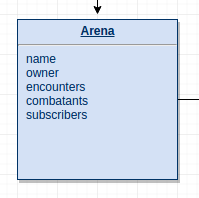
\includegraphics[scale=.75]{schema-arena}
		\caption{Arena Schema}
		\label{fig: Arena Schema }
	\end{figure}
	
	\paragraph{}This schema will hold basic Arena information: an Arena name (name), a reference to Arena's creator: (owner), a list of encounters that are contained in the arena (encounters), and a list of references to users that are subscribed to the (subscribers). The Arena acts as a hub, organizer and access or for every user and their encounters. Arena statistics are not directly maintained in the Area object itself but are compiled from the list of encounters that is contained in the encounters field. This allows the statistics as up to date as possible without constantly updating both area statistic and the encounter statistics when an encounter goes through a stat change.
	
	\subsection{Encounter Schema}
	\begin{figure}[H]
		\centering
		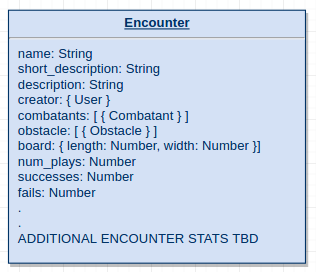
\includegraphics[scale=.75]{schema-encounter}
		\caption{Encounter Schema}
		\label{fig: Encounter Schema }
	\end{figure}
	Encounters created by a user will be saved in a encounter document using this schema. It will contain basic descriptive information: name, descriptions, creator. As well as physical details about the encounter itself: an array of obstacles, an array of combatants, board size. The encounter will also contain statistical information useful for both players and game masters: number of plays, success rate, most played class. This is  where statistical data is stored, these statistics will flow upward and be adjusted and displayed on other components such as arena statistics.
	\subsection{Combatant Schema}
	\begin{figure}[H]
		\centering
		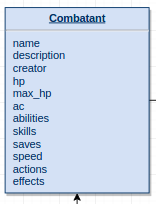
\includegraphics[scale=.9]{schema-combatant}
		\caption{Combatant Schema}
		\label{fig: Combatant Schema }
	\end{figure}
	This schema will be used to represent all combatants in an encounter, both player and non-player characters. All of the base stats for the combatant are stored in the document. All bonuses will be added after so it is easy to add and remove bonuses to combatant stats. Stat modifiers will also not be calculated using the respective modifier formula as well as adding additional bonuses from any effects the combatant has received from items, features and abilities. We designed the the schema this way to keep the database uncomplicated so it will be easier to edit and create new combatants. The combatant document will also contain a array of actions that the combatant can take on its turn. These actions will be displayed and selectable in the Battlefield sidebar on the combatants turn and combat.  All combatants will be assigned a reference to its creator. Most of the combatants at first implementation will be under Critical Encounters' user ID and they will be available to use for all users. This feature will also make it easy to implement creature and combatant sharing sometime in development or as a stretch goal.
	\subsection{Obstacle Schema}
	\begin{figure}[H]
		\centering
		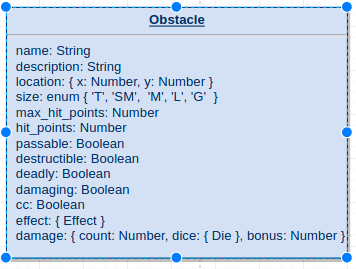
\includegraphics[scale=.9]{schema-obstacle}
		\caption{Obstacle Schema}
		\label{fig: Obstacle Schema }
	\end{figure}
	This schema contains data for non-combatant entities in an encounter, i.e. entities that do not have a turn in combat and do not roll initiative. Examples of obstacles are walls, traps, doors, inanimate objects, water, holes, and items. The schema outlines basic descriptive information information name, description and size, as well as a range of boolean values that describe the obstacle's role and interaction with players in combat. For example, a bottomless pit would have the deadly boolean set to true so any combatant that were to fall in it would die instantly. Walls on the other hand would have the passable boolean set to false, which will stop the AI pathfinder from choosing a path through walls. The obstacle will also have an array of Effects. These  effects would include any Crowd Control, Damage, Healing or Magical effects the obstacle might have. This includes damage for traps, half speed for traveling through brush, and magical healing aura from enchanted statures. The implementation of the effects may change to bettersuit the implementation of the AI combat and encounter flow.
	\subsection {Action Schema}
	\begin{figure}[H]
		\centering
		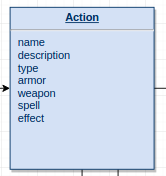
\includegraphics[scale=.9]{schema-action}
		\caption{Action Schema}
		\label{fig: Action Schema }
	\end{figure}
	The action schema contains data about actions combatants will be able to take on their turn. The actions stored in the database will be restricted to actions given gained from items, features, classes, and races. Actions available to all combatants, movement, disengage and dash for example will be hard coded for all combatants to avoid bloating the database. The purpose of an action document is to describe the action and its requirements. Little computational work will be done directly to the action document, instead it will be done with the action's effects.
	\subsection {Effect Schema}
	\begin{figure}[H]
		\centering
		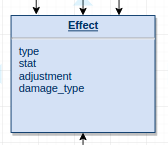
\includegraphics[scale=.9]{schema-effect}
		\caption{Effect Schema}
		\label{fig: Effect Schema }
	\end{figure}
	The effect schema will be were most of the computational data will be held. It will be held as reference by many other documents such as armor, weapons, and features. Effects adjust player stats like health, strength, and speed. They can apply a flat bonus or reduction, half, double or triple statistics, or apply a advantage or disadvantage to stat checks. The stat change will be described in the type
	\subsection {Spell Schema}
	\begin{figure}[H]
		\centering
		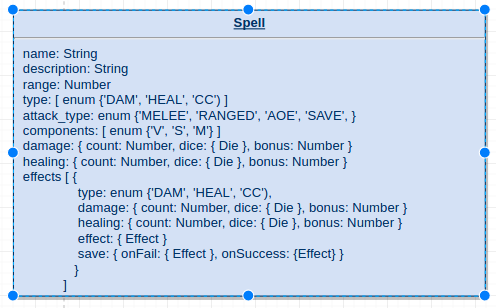
\includegraphics[scale=.9]{schema-spell}
		\caption{Spell Schema}
		\label{fig: Spell Schema }
	\end{figure}
	This schema describes a spell associated with a combatant action in game it contains description information as well as an array of the spells effects describes inside effect objects.We decided to construct a spell very modularly and easily customizable so that sometime in future development we can easily implement a to allow users to create and edit their own spells.Most of what the AI is going to interact with in a spell document is with the array of Effect objects.
	\subsection {Weapon Schema}
	\begin{figure}[H]
		\centering
		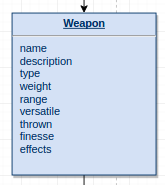
\includegraphics[scale=.9]{schema-weapon}
		\caption{Weapon Schema}
		\label{fig: Weapon Schema }
	\end{figure}
	This schema describes a weapon that can be equipped by a combatant. Weapons are referenced in actions and the data the weapon contains, their flat stats such as damage and range and their referenced effects. These effects are implemented by the AI the actions during combat.
	
	\subsection {Armor Schema}
	\begin{figure}[H]
		\centering
		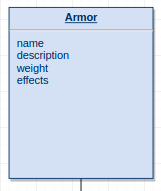
\includegraphics[scale=.9]{schema-armor}
		\caption{Armor Schema}
		\label{fig: Armor Schema }
	\end{figure}
	This schema describes an armor that can be equipped by a combatant. Armor is referenced in actions and the data the armor contains, their flat stats such as armor class and weight and their referenced effects. These effects are implemented by the AI the actions during combat.
	\newpage
	\section{Client Side Design}
	
	\subsection{URL and Routing}
	There are two options to font-end routing for using our stack: React-Router and Meteor's FlowRouter. Both implementations have their pros and cons but after some research and deliberation we have decided to use Meteor's FlowRouter. The notation and syntax for FlowRouter is much more clear and easier to learn. There haws also been a history of React-Router not playing too well with Meteor applications. 
	
	FlowRouter is relatively straight fore-ward and is composed of two main components, the URL and the action. In short when the URL is accessed by the browser the action is triggered. In our case the action method will most likely be a ReactLayout render call to render react components associated with that route to the view.
	
	Below is a routing example for the dashboard page of Critical Encounters:
	
	\begin{lstlisting}
	FlowRouter.route( '/dashboard', {
	name: 'dashboard',
	action() {
	ReactLayout.render( App, { yield: <DashBoard /> } );
	}
	});
	\end{lstlisting}
	
	\subsubsection { URL Routes}
	
	\begin{table}[H]
		\begin{center}
			\begin{tabular}{ |p{5cm}|p{7cm}|| } 
				\hline
				URL Route: & Purpose: \\
				\hline
				/dashboard & Routes users to dashboard page \\
				/account & Routes current user account information\\
				/encounter-finder/:query & Route to search result page accessible at anytime through the fixed header search bar  \\
				/arenas/:arenaName & Route to area with specified arena name  \\
				/encounters/:id & Route to encounter with specified id \\
				/battlefield/creator/:id & Enter Battlefield in creator mode with given encounter id \\
				/battlefield/player/:id & Enter Battlefield in player mode with given encounter id \\
				/battlefield/master/:id & Enter Battlefield in master mode with given encounter id \\	
				\hline
			\end{tabular}
		\end{center}
		\caption{URL Routes} \label{table: URL Routes}
	\end{table}
	
	\subsection{Battlefield Modes}
	\subsubsection{Game Mode}
	This is the main mode available in the Critical Encounters Battlefield. In this mode users will be able to play, simulate, and view and gather data about their own encounters as well as other user's.
	\subsubsection{Role: Player}
	Player is in control of a single player character and can either control his character directly in combat or apply an AI to his player character. every round the player will perform his/her character's actions on its turn. Once complete the AI will simulate all other combatant's turns and refresh the battlefield. Once the encounter is complete the player will be able to view his character's stats and results from the encounter.
	\subsubsection{Role: Game Master}
	Controls multiple combatants against a one or more player characters. The game master on each turn can choose to either simulate the combatant's turn or perform the actions on the combatant's turn manually using the AI. After the encounter has completed there the game master will be able to review the encounter stats and results.
	
	\subsubsection{Creation Mode}
	\subsubsection{Role: Creator}
	There is only one role available for the Creation Mode: the Creator role. In this mode the user will be able to design their own encounters using the Encounter Creator Tools. Users will be able to add obstacles and combatants, as well as customize the combatants stats and AI presets. Once the user has completed creating the encounter the user may either publish the encounter, and perform Encounter Validation process or keep the encounter private for personal or invite use.
	
	\newpage
	\subsection{Turn Structure / Order}
	Combat using the d20 System is composed of rounds in which each combatant in the encounter has one turn.  A round lasts 6 seconds in game time, during which all combatants act on their respective turns. Where a combatant's turn resides chronologically in a round is determined by the combatant's initiative roll (a combination of a dice roll and applicative bonuses). A turn it self is composed of 6 parts: Action(s), Bonus Action, Movement, Free Action, and Bonus Action, Reaction.
	\begin{itemize}
		\item Action
		\begin{itemize}
			\item The main action of a turn, every combatant has one or more per turn
			\item Ex. Attack, Cast a Spell, Dash, Disengage, Hide
		\end{itemize}
		\item Bonus Action
		\begin{itemize}
			\item An action gained by a feature, spell, or other abilities
			\item Ex: The Cunning Action feature allows a rogue to take a Bonus Action to hide, dash, or disengage
			\item Max one Bonus Action per turn
		\end{itemize}
		\item Movement
		\begin{itemize}
			\item Combatant can move the number of spaces equal to its speed (with applicaple bonuses) divided by five
			\item Some combatants also have swim and flight speeds that they can use as their movement action
			\item Multiple environmental restraints on this: Difficult terrain, attacks of opportunity
		\end{itemize}
		\item Free Action
		\begin{itemize}
			\item Interact with one object or environment 
			\item Ex: Open a door, you could draw your weapon
			\item interaction with more than one action requires the use of an action
		\end{itemize}
		\item Reaction
		\begin{itemize}
			\item Combatant has one of reaction in every round of combat
			\item Can happen anytime during the round, doesn't have to be combatant's turn
			\item Ex. Cast reaction spell, attack of opportunity
		\end{itemize}
	\end{itemize}
	
	\section {Testing}
	
	For our testing we will be using a combination of both manual and automated testing. Automated testing will be performed using ReactTestUtils which will allow us to rapidly test front-end components. There is also a Meteor test tool that can be used to test both the client and servers sides of the application.
	
	Most of our efforts when it comes to testing our application will center around testing the AI. Since the AI is the most complex and most important part of the application we are doing to test it extensively so that users are satisfied with the primary feature of our application. To this end, we are focusing our efforts on developing the Battlefield as it will serve as a very useful tool to view and test output from the AI. Below is the order in which  we plan to test the AI. 
	
	\begin{itemize}
		\item Movement
		\begin{itemize}
			\item Combatant movement to target
			\item Combatant movement to target around obstacles
			\item Combatant movement when target is unreachable
		\end{itemize}
		\item Attacks
		\begin{itemize}
			\item Combatant melee attack when target is within melee range
			\item Combatant ranged attack when has line of sight and is within range.
			\item Combatant melee attack when target is not in range but is in movement range
			\item Combatant ranged attack when target is not in range but is in movement range
		\end{itemize}
		\item Spells
		\begin{itemize}
			\item Melee spell
			\item Ranged single target spell
			\item Ranged AOE spell
			\item Ranged line spell
			\item Ranged cone spell
			\item Spell Type Priority
			\begin{itemize}
				\item Damage
				\item Healing
				\item Crowd Control
			\end{itemize}
		\end{itemize}
		\item Alternative actions
		\begin{itemize}
			\item Dash to better position or out of attack range
			\item Disengage when threat is too great
			\item Hide when high treat or better position
		\end{itemize}
	\end{itemize}
	
	Our plan for testing involving all components, both the search and profile layouts and the Battlefield, are summarized by the outline below:
	
	\begin{itemize}
		\item{UI}
		\begin{itemize}
			\item Ensure that UI fits most desktop sizes 
			\item Ensure that the search bar is fixed in the header on all pages
			\item Ensure that the encounter feed output links to the correct encounters under the correct category
			\item Ensure that the search bar always redirects to the search page
			\item Display all correct stat data in arena correctly
			\item Ensure all buttons are cursor responsive and perform their correct actions
			\item Ensure that reviews are posted immediately under encounters
		\end{itemize}
		\item Data
		\begin{itemize}
			\item Ensure that correct encounter data is gathered, parsed and available for use in the Arena page.
			\item Ensure that new data from encounters is processed correctly and updated in the arena and encounter statistics
			\item Ensure that correct data is loaded to the Battlefield sidebar for use in both creation and play modes
			\item Ensure all encounter lists are correct in the dashboard page
		\end{itemize}
	\end{itemize}

	
\end{document}